\section{Reconstruction}\label{sec:Reconstruction}

For the 3-D reconstruction of a scene a high-speed stereo sequence is captured with \textit{TimeBench} and this data is then analyzed and computed in MATLAB. The estimated extrinsic and intrinsic camera parameters are retrieved from the camera calibration from \autoref{sec:Calibration} with which the cameras' positions are now known in world coordinates. The pipeline of reconstruction is illustrated in \autoref{fig:ReconstructionPipeline}. The corresponding MATLAB \textit{depthEstimationFromStereoImages.m} is included in the digital appendix of this thesis.

\begin{figure}[htbp]
		\centering
		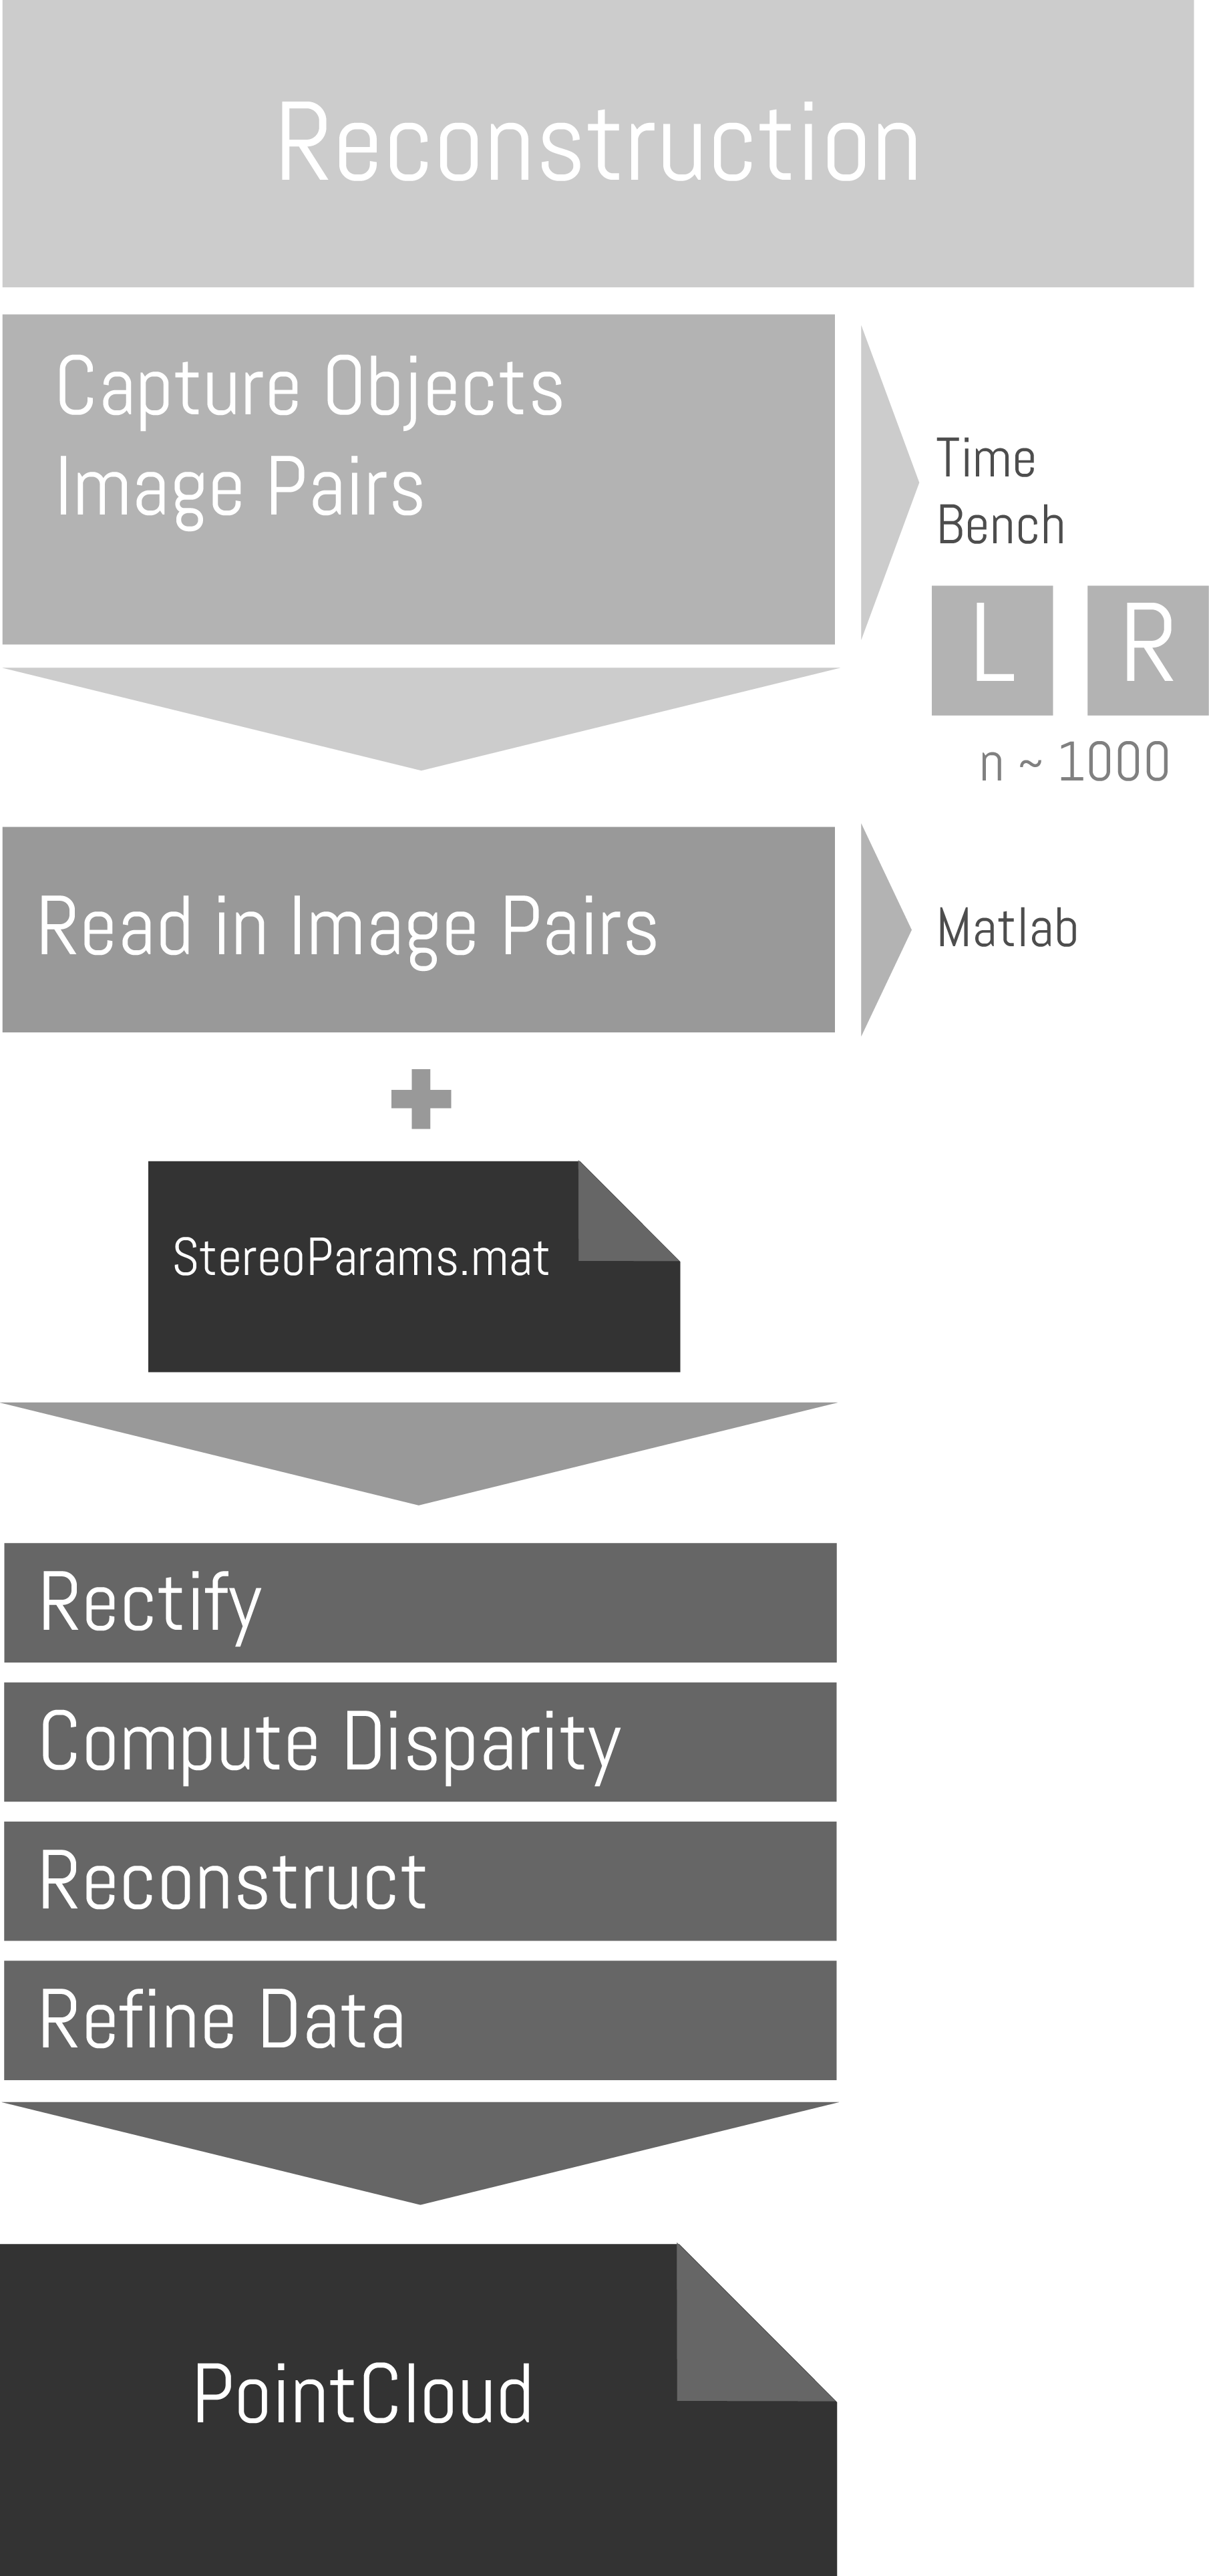
\includegraphics[width=0.6\textwidth]{figures/Reconstruction}
		\caption[Steps of the reconstruction in TimeBench and in MATLAB]{Steps of the reconstruction in TimeBench and in MATLAB, using a set of $n$ image pairs.}
		\label{fig:ReconstructionPipeline}
\end{figure}

\subsection{Capturing a Sequence of moving Objects in TimeBench}\label{ssec:CaptureReconstrSequence}
The capturing of a sequence of moving objects to be reconstructed follows the procedure as explained in \autoref{ssec:PatternSequence}. The cameras must be in the exact same position with the exact same adjustments as in the calibrated scene\footnote{Since it might not be possible to recreate the exact same set-up, the cameras should not be moved at all during the calibration and reconstruction procedure. The only entities which are allowed to be changed in terms of position are the lights.}.

The selection of objects which are later to be reconstructed (in the following simply called \textit{objects}) is an important step. The feature detection algorithms need enough different textures and forms in order to detect corresponding points. This topic is discussed in detail in the examples and in the results (\autoref{sec:ExperimentalResults}). The objects need to be brightly illuminated and should not cast too many shadows. They need to be in focus as well. It is recommended that objects be used which are asymmetrical and which have many different textures. Transparent objects should be avoided.

The cameras' frame rate is increased to 500 fps and the sequence is captured in \textit{TimeBench}. Instead of saving only single images, the whole sequence (or the part of interest) is exported (as \textit{bmp}-files). It is of course important to save exactly the same frames of both output data sets. The ring buffer allows a number of approximately 1000 \textit{bmp}-images from each camera to be captured, which results in 2000 images to be processed.

\begin{figure}[htbp]
		\centering
		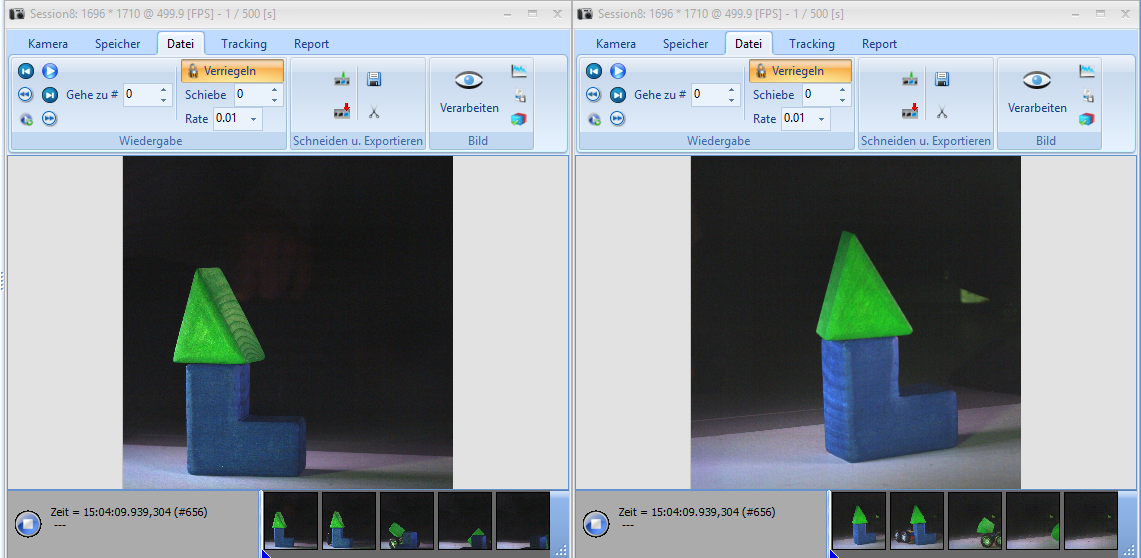
\includegraphics[width=1.0\textwidth]{figures/timebenchSequence}
		\caption[Image sequence of a captured scene in TimeBench]{Image sequence of a captured scene in TimeBench (\textit{source: software TimeBench owned by} \cite{Optronis.2016}).}
		\label{fig:timebenchSequence}
\end{figure}

\subsection{3-D Reconstruction in MATLAB}\label{ssec:ReconstrMatlab}
\paragraph{Loading images and stereo parameters}
After loading the \textit{stereoParameters}\footnote{Stereo parameters can be gained in different ways. In this case they are the output of the Stereo Camera Calibration Toolbox from MATLAB.} object the image sequences needs to be saved in two variables.
For a better overview the following procedures will be explained for only one pair of images, $I1$ (left camera) and $I2$ (right camera). In case of a whole image sequence the steps need to be repeated in a loop for all images.
\begin{lstlisting}[caption={Load stereoParams and images.}]
 load('stereoParams.mat');
 I1 = imread('D:\left.bmp');
 I2 = imread('D:\right.bmp');
\end{lstlisting}

\paragraph{Rectification}
The two images must now be rectified (the mathematical background is summarized in \autoref{ssec:RectificationDisp}). The MATLAB function \textit{rectifyStereoImages}\footnote{The documentation of the MATLAB object can be found at \url{http://www.mathworks.com/help/vision/ref/rectifystereoimages.html}.} returns the undistorted and rectified images $J1$ and $J2$ from $I1$ and $I2$, taking the estimated stereo parameters into account. If the stereo parameters are not yet estimated (which means the cameras are uncalibrated) the images can still be rectified by first searching \textit{features}, for example with the \textit{detectSURFFeatures} function and then find point correspondeces in the images. The function \textit{estimateUncalibratedRectification} lets one compute the rectification transformations. After this the images can be rectified with the same function\footnote{An example for the rectification of images from uncalibrated cameras can be found at: \url{http://www.mathworks.com/help/vision/examples/uncalibrated-stereo-image-rectification.html}.}. 

\begin{lstlisting}[caption={Image rectification.}]
[J1,J2] = rectifyStereoImages(I1,I2, stereoParams);
figure
imshowpair(J1, J2, 'montage');
title('Rectified Images');
\end{lstlisting}

\paragraph{Disparity map}
The disparity map\footnote{The documentation of disparity can be found at \url{http://www.mathworks.com/help/vision/ref/disparity.html}}\index{Disparity map} returns the disparities for corresponding pixels of stereo images as an $M$-by-$N$ 2D grayscale image with the same size as the input data, which are the rectified images $J1$ and $J2$. The \textit{disparityRange} depends on the the cameras' baseline and the distance between the cameras and the objetcs. To get better results the rectified images can be viewed as a \textit{stereo anaglyph} and the distance between two corresponding images can be measured with the \textit{Distance tool}. According to the results the disparity range can be modified, whereby the bigger the range the bigger the computation time. The numbers of the range must be divisible by 16 with an array range of less than 1629.  

\begin{lstlisting}[caption={Display disparity map.}]
disparityRange = [0 1600];
disparityMap = disparity(rgb2gray(J1),rgb2gray(J2),'DisparityRange',disparityRange); 
figure
imshow(disparityMap, disparityRange);
title('Disparity Map');
colormap jet
colorbar
\end{lstlisting}

\begin{figure}[htbp]
		\centering
		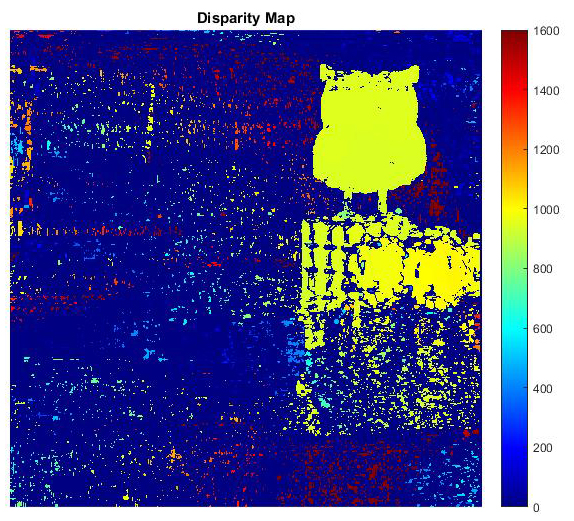
\includegraphics[width=0.6\textwidth]{figures/DisparityMap}
		\caption[Output of the disparity function]{The output of the disparity function displays the disparity map.}
		\label{fig:DisparityMap}
\end{figure}

\paragraph{Reconstruct scene}
The scene can now be reconstructed with the disparity map. The function \textit{reconstructScene}\footnote{See the MATLAB documentation at \url{http://www.mathworks.com/help/vision/ref/reconstructscene.html}.} returns the detected and computed 3-D world point coordinates in a $M$-by-$N$-by-$3$ array - a so called \textit{point cloud}\index{Point cloud}. Due to this fact the output displays absolute values and can be used to measure the real sizes of the reconstructed objects. The point cloud represents the 3-D world points relative to camera 1 in the stereo system computed with the camera calibration. The disparity map's data type determines the type of the point cloud (\textit{single} or \textit{double}). The point clouds of the set of image pairs can be displayed in a point cloud \textit{player} instead of only showing one point cloud.

\begin{lstlisting}[caption={Reconstruction of the scene, saved as a point cloud.}]
points3D = reconstructScene(disparityMap, stereoParams);
points3D = points3D ./ 1000;
ptCloud = pointCloud(points3D, 'Color', J1);
player3D = pcplayer([-3, 3], [-3, 3], [0, 8], 'VerticalAxis', 'y', ...
    'VerticalAxisDir', 'up');
view(player3D, ptCloud);
\end{lstlisting}

\begin{figure}[htbp]
		\centering
		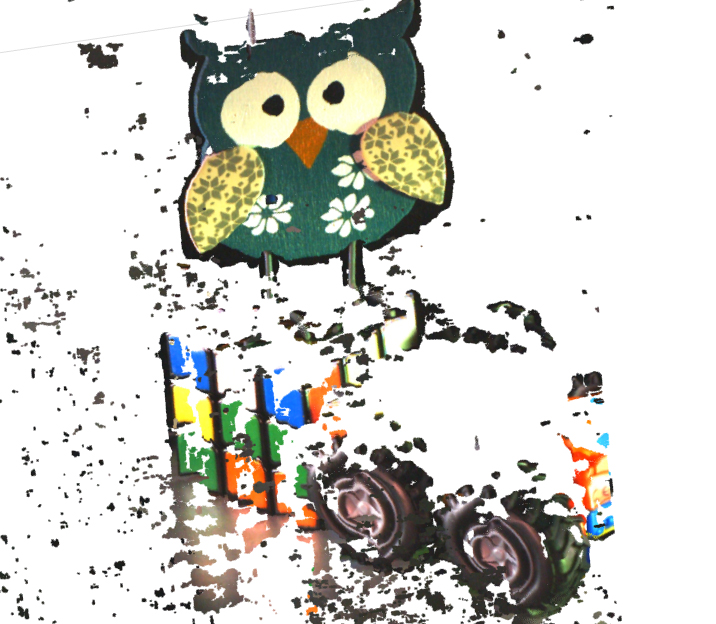
\includegraphics[width=0.6\textwidth]{figures/PointCloud}
		\caption[Zoom into the point cloud of the reconstructed scene]{Zoom into the point cloud of the reconstructed scene.}
		\label{fig:PointCloud}
\end{figure}

\subsection{Data Refinement}\label{ssec:DataRefinement}
Obviously the scene reconstruction is far from ideal. A noisy or incorrect output can have different causes. If an error in the camera calibration can be excluded, the feature detection is likely to be not accurate enough to get a good result. 

\note{Since most of the filters needs to \enquote{run} through the whole array of the point cloud the processes take some time. For one point cloud this might be acceptable, but for the package of point clouds produced by a whole sequence of stereo images it is highly time-consuming.}

\paragraph{Filter out distances}
The first step should be to single out the objects from all noises which were detected around them and which are not interesting for the analysis. For this, two separate MATLAB files were written: the \textit{reducePtCData.m} and the \textit{filterOutPtCDist.m}.

The first file reduces the point cloud data by deleting \textit{NaN}- and \textit{inf}-data values. The output point cloud is unsorted and a lot smaller than the original one.

The second file takes this point cloud and filters out the distances which are defined by a so called \textit{axis-aligned bounding box}\index{Axis-aligned bounding box}. The specialty of this kind of bounding box is that it can be defined by only two 3-D vectors for the minimum and maximum coordinates which should still be in the scene. With this it can be checked rather easily if a point is inside or outside the axis-aligned bounding box. The point cloud points outside of the box are deleted (\cite[p.216 et seq.]{Gregory.2014}).

\paragraph{Denoise}
MATLAB has a built-in function to decrease the noise of point clouds: \textit{pcdenoise}\footnote{The documentation can be found at \url{http://www.mathworks.com/help/vision/ref/pcdenoise.html}.}. It removes \textit{outliers} and was not efficient in the experiments of this thesis. 

\paragraph{Bundle adjustment}
The \textit{Bundle adjustment}\index{Bundle adjustment} in computer vision is a way to minimize re-projection errors. It is only efficient if enough camera views are provided and is therefore often used in \textit{Structure from Motion}\index{Structure from Motion} algorithms, where a bundle of views from different angles of an object is captured (\cite[p.320 et seq.]{Szeliski.2011} and \cite[p.322 et seq.]{Luhmann.2014}).

Matlab provides a built-in method that refines camera poses and 3D points: the \textit{bundleAdjustment}\footnote{See a full description of the method at \url{mathworks.com/help/vision/ref/bundleadjustment.html}.}. At this point it should be mentioned that the code for this method is rather sparsely documented, which could make the usage of the built-in method tedious. However, there are a lot more solutions to choose from provided by the community\footnote{for example \url{https://github.com/tikroeger/BA_Matlab}.}. The bundle adjustment was not efficient in the experiments.

\subsection{Export}\label{ssec:Export}
The refined cloud object can be analyzed and reused in MATLAB. But to process and rework the 3-D model it is sometimes easier to export the point cloud as a mesh and to import it into another program. MATLAB provides the function \textit{pcwrite}\footnote{The description of the method can be found at \url{http://mathworks.com/help/vision/ref/pcwrite.html}} to write a 3-D point cloud into a \textit{PLY}-file. It can be chosen between the \textit{binary} or the \textit{ascii} format, whereas the former saves space. 

\begin{lstlisting}[caption={Export of the point cloud into a PLY file with binary format.}]
pcwrite(ptCloud,'stillOwl','PLYFormat','binary');
\end{lstlisting}

The exported point cloud can be for example imported into the software \textit{MeshLab}\index{MeshLab}. MeshLab\footnote{The tool was developed with the support of the 3D-CoForm project, which aimed to establish a universal state-of-the-art in 3-D-digitisation and 3-D-documentation. The research reports and other information can be found at \url{http://www.3d-coform.eu/}.} is open source and is specialized in processing and editing of unstructured 3-D meshes (\cite{Meshlab.2016}).